\chapter{Implementacija}

Kompletna implementacija napisana je u programskom jeziku \textit{Python} koji je odabran zbog svoje jednostavnosti, sažetosti, fleksibilnosti, neovisnosti o operacijskom sustavu, te velikoj popularnosti. Postoji veliki broj dobro dokumentiranih i iznimno korisnih biblioteka od kojih se za problematiku ovog rada izdvajaju biblioteke za oblikovanje i učenje dubokih modela (\textit{PyTorch}), biblioteka za iznimno brzo i učinkovito provođenje matematičkih operacija (\textit{Numpy}), te biblioteka za jednostavnu interakciju agenata i implementiranih okolina s kojima agent interaktira i dobiva povratnu informaciju (\textit{OpenAI Gym}).

Implementirani su duboki modeli prethodno predstavljenih algoritma dubokog Q učenja, dvostrukog dubokog Q učenja, te prednosnog akter-kritičara. Agenti u svojoj implementaciji interaktiraju s okolinama CartPole i Breakout.

\section{Moduli}

Implementacija je podijeljena u nekoliko modula: modul za generičko instanciranje dubokih modela, modul za generičku serijalizaciju i deserijalizaciju objekata (spremanje i učitavanje agenata), modul za \textit{OpenAI Gym} omotače i modul u kojem se nalazi implementacija agenata i algoritama.

\subsection{Instanciranje dubokih modela}

Modul \texttt{networks} sastoji se od metoda i struktura koje omogućuju generičko instanciranje dubokih modela, točnije unaprijednih potpuno povezanih modela i konvolucijskih modela opisanih u poglavlju \nameref{chap:duboki-modeli}. Prilikom poziva metode za instanciranje unaprijedne potpuno povezane mreže kao argument predaje se lista cijelih brojeva koje predstavljaju dimenzije pojedinih slojeva odvojenih nelinearnom aktivacijskom funkcijom ReLU (kao što je prikazano odsječkom \ref{lst:custom-fc}).

\begin{listing}[H]
    \caption{Generičko instanciranje unaprijedne potpuno povezane mreže}
    \inputminted{python}{snippets/custom-fc.py}
    \label{lst:custom-fc}
\end{listing}

S druge strane, pri instanciranju konvolucijske neuronske mreže, za definiranje atributa konvolucijskog sloja koristi se posebna struktura \texttt{CnnStructure} \ref{lst:cnn-structures} koja definira broj ulaznih i izlaznih kanala, dimenziju jezgre (slobodnih parametara koje učimo), veličinu koraka i nadopunu. Nakon konvolucijskog sloja provodi se nelinearnost aktivacijskom funkcijom ReLU. Na posljetku, značajke se transformiraju u vektor i prosljeđuju potpuno povezanom sloju. Pri prijelazu iz konvolucijskog sloja u potpuno povezani sloj, potrebno je točno izračunati broj parametara koji se prenose iz jednog sloja u drugi. Umjesto iscrpnog računanja, broj parametara je određen tako da se napravio jedan unaprijedni prolaz kroz definirane konvolucijske slojeve. Generični poziv funkcije za instanciranje konvolucijske neuronske mreže prikazan je odsječkom \ref{lst:custom-cnn}. 

\begin{listing}[H]
    \caption{Struktura za definiranje atributa konvolucijskog sloja}
    \inputminted{python}{snippets/structures.py}
    \label{lst:cnn-structures}
\end{listing}

Svi parametri konvolucijskog i potpuno povezanog sloja inicijalizirani su koristeći Kaiming uniformnu distribuciju koja u obzir uzima funkciju nelinearnosti koju koristimo.

\begin{listing}[H]
    \caption{Generičko instanciranje konvolucijske neuronske mreže}
    \inputminted{python}{snippets/custom-cnn.py}
    \label{lst:custom-cnn}
\end{listing}

\subsection{Serijalizacija i deserijalizacija agenata}

Modul \texttt{serialization} sadrži metode za učitavanje i spremanje \textit{Python} objekata, točnije serijalizaciju objekata u tok okteta podataka \engl{byte stream} i njegovu deserijalizaciju. Za samo spremanje koriste se pomoćne funkcije biblioteke \textit{PyTorch} (\texttt{torch.save} i \texttt{torch.load}) koje u internoj implementaciji koriste biblioteku za serijalizaciju i deserijalizaciju - \textit{Pickle}. U implementaciji koristimo navedene funkcionalnosti kako bi sačuvali i učitali parametre naučenih dubokih modela. 

\subsection{Omotači}

Prema uzoru na biblioteku \textit{Stable Baselines3} i članke koji opisuju dobre i kvalitetne pristupe pri rješavanju problema podržanog učenja \cite{DQL}, modul \texttt{wrappers} sadrži zbirku implementiranih \textit{OpenAI Gym} omotača. Svi korišteni omotači prilagođeni su uporabi na \textit{Atari} okolinama. Ideja je da originalnu okolinu omotamo u strukture koje omogućavaju izmjenu elemenata postojećeg okruženja bez potrebe za mijenjanjem originalnog koda. Omotač \texttt{WarpFrame} koristeći biblioteku \textit{cv2} (\textit{OpenCV}) skalira sliku okoline na okvir dimenzija $84 \times 84$ i pretvara RGB vrijednosti piksela u nijanse sive boje \engl{grayscale}, kao što je i prikazano na slici \ref{fig:warp-frame}.

\begin{figure}[H]
    \centering
    \frame{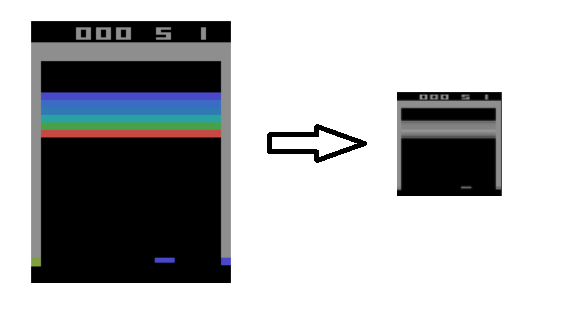
\includegraphics[width=8cm]{assets/warp-frame.png}}
    \caption{Breakout okoline prije i nakon korištenja omotača \texttt{WarpFrame}}
    \label{fig:warp-frame}
\end{figure}

Obratimo pažnju ponovno na prikaz \ref{fig:warp-frame}. Dimenzije (širina - $W$, visina - $H$ i broj kanala - $C$) slike lijevo su $160 \times 210 \times 3$ a slike desno $84 \times 84 \times 1$. Iz razloga što okolina vraća slike u dimenziji $H \times W \times C$, a \textit{PyTorch} konvolucijski sloj prima dimenzije oblike $C \times H \times W$, napravljen je posebni omotač \texttt{TransposeImageObs} koji uređuje dimenzije.

Omotači mogu poslužiti i za ugrađivanje stohastike u atari okruženjima kao što je i opisano u poglavlju \ref{chap:determinizam}. Omotač \texttt{NoopResetEnv} osigurava da na početku epizode okolina ignorira akcije agenta (tehnika \textit{initial no-ops}). Omotač \texttt{MaxAndSkipEnv} provodi tehniku \textit{frame skipping} i $n$ puta vraća istu povratnu informaciju agentu. 

Od ostalih korisnih omotača, bitno je spomenuti omotač \texttt{ClipRewardEnv} ograničava nagrade okoline na vrijednosti $ \{ -1, 0, 1 \} $, \texttt{FireResetEnv} koji na početku epizode izvršava operaciju \texttt{FIRE}, \texttt{BatchedPytorchFrameStack} koji u kombinaciji s \texttt{SubprocVecEnv} osigurava istovremeno izvođenje nekoliko instanci okruženja koristeći biblioteku \textit{multiprocessing} \cite{SB3}.

\section{Implementacijski detalji}

\subsection{Duboko Q učenje}

Na samom početku izvođenja algoritma potrebno je napuniti spremnik za ponavljanje $D$ i u njega pohraniti sve akcije, stanja i nagrade koje je agent poduzeo od početka. Iz tog razloga korisno je napraviti strukturu koja predstavlja uređenu $n$-torku \texttt{Transition} i razred \texttt{ReplayMemory} kao što je prikazano kodom \ref{lst:replay-memory}. Razred interno za pohranu koristi kolekciju \texttt{deque} \engl{Doubly Ended Queue} koji se više preferira od listi zbog bržih operacija unosa i brisanja s početka i kraja reda. Kapacitet spremnika za ponavljanje određen je parametrom \texttt{capacity}. Razred sadrži metode za ubacivanje podataka i nasumično uzorkovanje određenog broja prijelaza.

\begin{listing}[H]
    \caption{Instanciranje neuronskih mreža}
    \inputminted{python}{snippets/replay-memory.py}
    \label{lst:replay-memory}
\end{listing}

Slijedi instanciranje dviju neuronskih mreža: mreže koja prati trenutnu politiku i provodi stalno ažuriranje parametara \texttt{online_net} (s parametrima $\theta$), i mreže koja prati ciljanu politiku \texttt{target_net} (s parametrima $\theta^-$). Nakon instanciranja, obje mreže trebaju imati jednaku vrijednost parametara. Navedeno je prikazano odsječkom koda \ref{lst:dqn-nets}.

\begin{listing}[H]
    \caption{Struktura spremnika za ponavljanje}
    \inputminted{python}{snippets/dqn-nets.py}
    \label{lst:dqn-nets}
\end{listing}

U svakom koraku potrebno je odabrati iduću akciju koju će agent poduzeti. Provodimo tehniku istraživanja (pritom odabiremo nasumičnu akciju) i odabira akcije s najvećom Q vrijednošću (potencijalno najkorisniju akciju). Opisana strategija \textit{epsilon-greedy exploration} prikazana je kodom \ref{lst:dqn-actions}.

\begin{listing}[H]
    \caption{Implementacija \textit{epsilon-greedy exploration} strategije}
    \inputminted{python}{snippets/dqn-actions.py}
    \label{lst:dqn-actions}
\end{listing}

Gubitak se izračunava postupkom \ref{lst:dqn-loss} prema formuli \ref{md:dqn-loss}. Prvo se provodi unaprijedni prolaz nad mrežom \texttt{target_net} i pritom se dobivaju vrijednosti $Q(s_{t+1}, a; \theta^-)$. Računa se njihova maksimalna vrijednost i skalira hiperparametrom \texttt{gamma}. Provodi se unaprijedni prolaz nad mrežom \texttt{online_net} (vrijednosti $Q(s_t, a_t; \theta)$) i od prikupljenih vrijednosti računa huberov gubitak za kojeg se pokazalo da je bolji od srednje kvadratne pogreške \engl{Mean Squared Error} zbog manje osjetljivosti na odustupanja \engl{outliers}. Nakon izračuna gubitka, provodi se izračun gradijenta i ažuriranje parametara \texttt{online_net} mreže. Nakon što prođe određeni broj koraka, provodi se zamjena vrijednosti parametara, odnosno ažuriranje parametara \texttt{target_net} mreže.

\begin{listing}[H]
    \caption{Izračun gubitka dubokog Q učenja}
    \inputminted{python}{snippets/dqn-loss.py}
    \label{lst:dqn-loss}
\end{listing}

\subsection{Dvostruko duboko Q učenje}

Algoritam dvostrukog dubokog Q učenja rješava problem precjenjivanja vrijednosti funkcije akcije. Razlika između njega i algoritma dubokog Q učenja očituje se u izrazu i računanju funkcije gubitka \ref{md:ddqn-loss}. Upravo to je bio i cilj - riješiti problem precjenjivanja pritom ne mijenjajući osnovni kostur algoritma. Prema algoritmu, izračun funkcije gubitka počinje unaprijednim prolazom kroz \texttt{online_net} mrežu i dobivanjem vrijednosti $Q(s_{t+1}, a, \theta)$. Nad dobivenom vrijednostima provodimo operaciju $\argmax$ - uzimamo najveće Q vrijednosti i zapamtimo akcije kojima su one pridružene. Nad \texttt{target_net} mrežom računamo unaprijedni prolaz i Q vrijednosti izračunate s parametrima $\theta^-$ pridružujemo ranije zapamćenim akcijama. Daljnje računanje istovjetno je postupcima u dubokom Q učenju - izračun $Q(s_t, a_t; \theta)$, huberovog gubitka, gradijenta i ažuriranje parametara $\theta$ \texttt{target_net} mreže 

\begin{listing}[H]
    \caption{Izračun gubitka dvostrukog dubokog Q učenja}
    \inputminted{python}{snippets/ddqn-loss.py}
    \label{lst:ddqn-loss}
\end{listing}

\subsection{Prednosni akter-kritičar}

Implementacija prednosnog akter-kritičar algoritma započinje konstruiranjem dubokog modela s idejom da i akter i kritičar dijele sve slojeve iste neuronske mreže osim posljednjeg sloja. Dimenzija izlaznog sloja aktera odgovara broju akcija koje su akteru na raspolaganju u određenoj okolini, dok istovremeno kritičar ima samo jedan izlaz koji odgovara procjeni funkcije stanja. Odsječak koda \ref{lst:a2c-net} prikazuje inicijalizaciju potpuno povezanog dubokog modela s dva različita izlazna sloja.

\begin{listing}[H]
    \caption{Inicijalizacija potpuno povezanog dubokog modela algoritma akter-kritičar}
    \inputminted{python}{snippets/a2c-net.py}
    \label{lst:a2c-net}
\end{listing}

Prilikom unaprijednog prolaza, potrebno je prvo izračunati izlaz iz zajedničkog dijela mreže i potom rezultat provući kroz sloj aktera i sloj kritičara. Akter izračunava vjerojatnost poduzimanja akcija, dok kritičar procjenjuje funkciju stanja. Odsječak unaprijednog prolaza prikazan je kodom \ref{lst:a2c-forward}.

\begin{listing}[H]
    \caption{Unaprijedni prolaz algoritma akter-kritičar}
    \inputminted{python}{snippets/a2c-forward.py}
    \label{lst:a2c-forward}
\end{listing}

Pri svakoj iteraciji potrebno je odrediti akciju koju će izvršiti agent. Taj odabir akcije prikazan je kodom \ref{lst:a2c-action}. Unaprijednim prolazom mreže dobijemo vjerojatnost poduzimanja svake od mogućih akcija i vrijednost funkcije stanja. Agent će poduzeti akciju koja ima najveću vjerojatnost. Dobivena nagrada, vjerojatnost akcija i vrijednost stanja pohranjuju se sve do kraja epizode kada se provodi evaluacija, izračunava gubitak, provodi izračun gradijenata i ažuriranje parametara.

\begin{listing}[H]
    \caption{Odabir akcije i pohrana podataka za evaluaciju algoritma \textit{A2C}}
    \inputminted{python}{snippets/a2c-action.py}
    \label{lst:a2c-action}
\end{listing}

Konačno, na kraju epizode provodi se postupak evaluacije prikupljenog znanja \ref{lst:a2c-eval}. Prvo za svaki korak izračunavamo diskontni povrat od stanja $t$ pa sve do kraja epizode (vrijednost $R_t$). Slijedi računanje gubitka. Za svaku iteraciju izračunava se funkcija prednosti \ref{md:advantage-function-with-return}. Funkcija prednosti je razlika izračunatih diskontnih povrata i procjene funkcije stanja koju je kritičar procijenio prilikom poduzimanja svake akcije \ref{lst:a2c-action}. Nadalje, gubitak aktera i kritičara računa se prema izrazima \ref{md:a2c-actor-loss} i \ref{md:a2c-critic-loss}. Gubitci se zbroje, provede se izračun gradijenata i ažuriranje parametara dubokog modela.

\begin{listing}[H]
    \caption{Evaluacija aktera i kritičara u algoritmu \textit{A2C}}
    \inputminted{python}{snippets/a2c-eval.py}
    \label{lst:a2c-eval}
\end{listing}

\section{Rezultati agenata CartPole okoline}

Učenje dubokih modela izvršavalo se na grafičkoj kartici \textit{NVIDIA Quadro T1000 with Max-Q Design} uz omogućeno CUDA ubrzanje. Hiperparametri agenata koji su u potpunosti ručno implementirani, navedeni su u dodatku \ref{appendix:cartpole-hiperparams}. Agenti su učeni na okolini \texttt{CartPole-v1} u kojoj je posebnim omotačem specificirano da epizoda može trajati najviše $500$ koraka što je jedan od kriterija zaustavljanja. S druge strane, želimo naučiti agente da budu dugoročno što bolji u okolini. Bez obzira na duljinu epizode, želi se postići da agent što duže u okolini može balansirati štap. Iz tog razloga, prilikom učenja maknuto je ograničenje duljine epizode - na taj način posebno nagrađujemo uspješne dugoročne pokušaje agenta.

\begin{listing}[H]
    \caption{Izraz za računanje kumulativne nagrade}
    \inputminted{python}{snippets/cumulative_reward.py}
    \label{lst:cum-rew}
\end{listing}

Krivulje prikazane na slici \ref{fig:cartpole-cumulative-reward} prikazuju kumulativni iznos nagrada u odnosu na broj iteracija. Kumulativni iznos nagrada računa se prema formuli prikazanoj odsječkom koda \ref{lst:cum-rew}. Kao što je iz grafa vidljivo, \textit{A2C} algoritam daje najbolje rezultate. Potrebno mu je manje vremena za učenje i osim ponekih oscilacija, poprilično je stabilan. Promatrani \textit{A2C} agent koristi relativno veliki iznos stope učenja ($0.03$) i samim time brže konvergira, no i ako smanjimo stopu učenja, algoritam se puno brže uči i njegova krivulja kumulativnog iznosa nagrada je stabilnija. Algoritmi koji se temelje na Q učenju su nestabilniji i zahtijevaju duže vrijeme učenja. Iznos kumulativne nagrade (u kasnijim stadijima učenja kada je parametar $\epsilon$ mali) posebno narušava odabir nasumične akcije zbog koje agent nekada poduzme akcije od kojih se ne može oporaviti. No zapravo, to nam i odgovara. Želimo da se agent nauči snalaziti u nepredvidivim i nepovoljnim situacijama.

\begin{figure}[H]
    \centering
    \frame{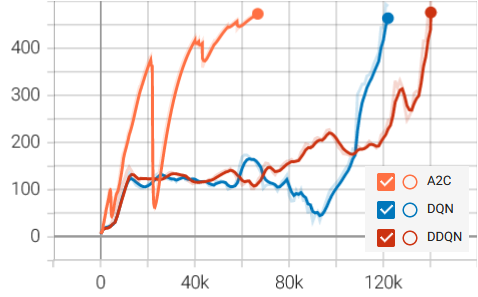
\includegraphics[width=9cm]{plots/cartpole-cumulative-reward.png}}
    \caption{Kumulativna nagrada po broju iteracija okolini CartPole}
    \label{fig:cartpole-cumulative-reward}
\end{figure}

\begin{figure}[H]
    \centering
    \frame{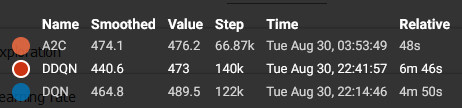
\includegraphics[width=10cm]{plots/cartpole-cm-stats.png}}
    \caption{Statistike agenata pri najvećoj vrijednosti kumulativne nagrade CartPole okoline}
    \label{fig:cartpole-stats}
\end{figure}

Također, prilikom mnogobrojnog pokretanja funkcije treniranja i opažanja ponašanja agenata, primijeti se da algoritam dvostrukog dubokog Q učenja nije primjetno bolji od njegove osnovne inačice algoritma. Vjerojatno je razlog taj što je riječ o jednostavnijoj okolini s relativno malim brojem dostupnih akcija i moguće je da ne dođe do prevelikog precjenjivanja funkcije akcije. Gledajući graf prosječne vrijednosti funkcije gubitka po broju iteracija \ref{fig:cartpole-loss} vidljivo je da agent dvostrukog dubokog Q učenja ima manji gubitak od svoje osnovne inačice što znači da se u zadanom vremenu bolje prilagodio okolini.

\begin{figure}[H]
    \centering
    \frame{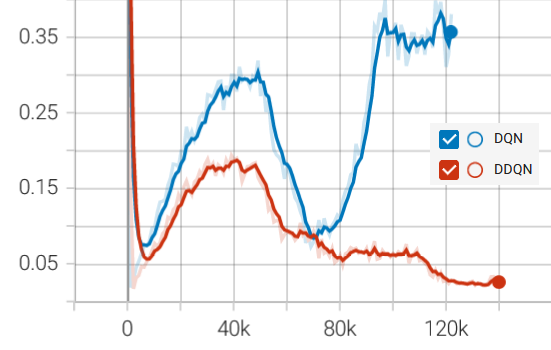
\includegraphics[width=9cm]{plots/cartpole-loss.png}}
    \caption{Prosječna vrijednost funkcije gubitka po broju iteracija u okolini CartPole}
    \label{fig:cartpole-loss}
\end{figure}

\section{Rezultati agenata Breakout okoline}

Učenje dubokih modela također se izvršavalo na grafičkoj kartici \textit{NVIDIA Quadro T1000 with Max-Q Design} uz omogućeno CUDA ubrzanje. Hiperparametri agenata navedeni su u dodatku \ref{appendix:breakout-hipperparams}. Učenje se provodilo na okolini \texttt{ALE/Breakout-v5}. Okolina je umotana u omotače koji pretvaraju RGB vrijednosti piksela u nijanse sive boje, skaliraju sliku na dimenziju $84 \times 84$, ograničavaju nagradu okoline na vrijednosti $\{-1, 0, 1\}$, provode stohastičke tehnike \textit{initial no_ops} i \textit{frame skipping}, te provode istovremeno treniranje nekoliko instanci okoline.

Agenti dubokog Q učenja i dvostrukog dubokog Q učenja su u potpunosti ručno implementirani, dok je za učenje prednosnog akter-kritičar agenta korištena biblioteka \textit{Stable Baselines3}. Zbog različitih implementacijskih detalja nije moguće napraviti direktnu usporedbu iznosa kumulativnih nagrada tijekom treniranja. 

Za razliku od okoline CartPole gdje dvostruko duboko Q učenje i njegova osnovna inačica nisu imali značajnijih odstupanja u postupku treniranja, okolina Breakout pokazala je korisnost i svrhu algoritma dvostrukog dubokog Q učenja. Upravo to prikazuju i grafovi \ref{fig:breakout-avg-ep-len} i \ref{fig:breakout-avg-rew}.

\begin{figure}[H]
    \centering
    \frame{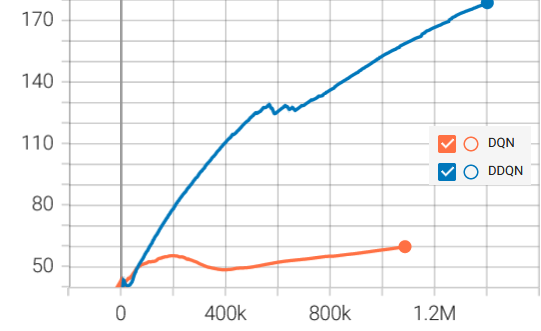
\includegraphics[width=9cm]{plots/breakout-avg-ep-len.png}}
    \caption{Prosječna duljina života agenta po epizodi u okolini Breakout}
    \label{fig:breakout-avg-ep-len}
\end{figure}

\begin{figure}[H]
    \centering
    \frame{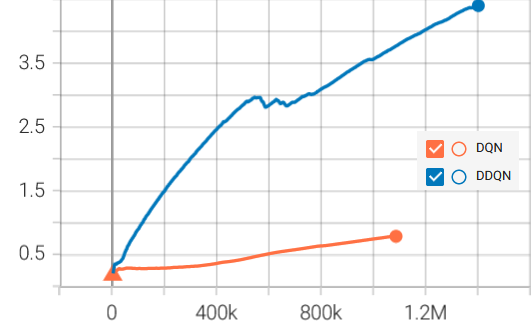
\includegraphics[width=9cm]{plots/breakout-avg-rew.png}}
    \caption{Prosječna vrijednost skalirane nagrade po epizodi u okolini Breakout}
    \label{fig:breakout-avg-rew}
\end{figure}

\begin{figure}[H]
    \centering
    \frame{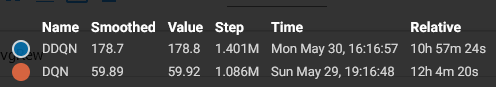
\includegraphics[width=10cm]{plots/breakout-stats.png}}
    \caption{Statistike agenata pri najvećoj vrijednosti nagrade Breakout okoline}
    \label{fig:breakout-stats}
\end{figure}

Agent algoritma prednosnog akter-kritičara naučen je koristeći biblioteku \textit{Stable Baselines3} koja je opisana u poglavlju \ref{chap:sb3}. Sama okolina omotana je gotovim omotačima koristeći pomoćnu funkciju \texttt{make_atari_env}. Implementacija biblioteke razlikuje se od prethodno opisane ručne implementacije i zbog toga performanse učenja nije moguće direktno usporediti. Informacije o prosječnoj vrijednosti duljine epizode po epizodi i prosječnoj vrijednosti nagrade po epizodi prikazane su na grafovima \ref{fig:breakout-a2c-ep-len-mean} i \ref{fig:breakout-a2c-ep-rew-mean}.

\begin{figure}[H]
    \centering
    \frame{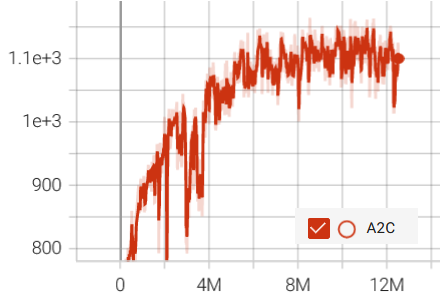
\includegraphics[width=9cm]{plots/breakout-a2c-ep-len-mean.png}}
    \caption{Prosječna vrijednost duljine epizode po epizodi algoritma \textit{A2C} u okolini Breakout}
    \label{fig:breakout-a2c-ep-len-mean}
\end{figure}

\begin{figure}[H]
    \centering
    \frame{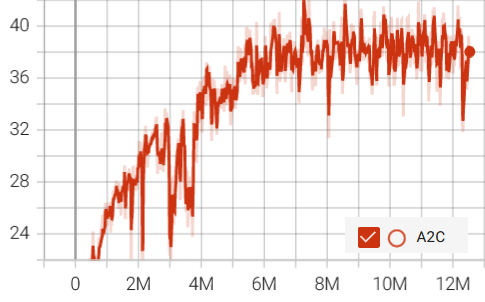
\includegraphics[width=9cm]{plots/breakout-a2c-ep-rew-mean.png}}
    \caption{Prosječna vrijednost nagrade po epizodi algoritma \textit{A2C} u okolini Breakout}
    \label{fig:breakout-a2c-ep-rew-mean}
\end{figure}

Naučene agente možemo direktno usporediti evaluacijom tako da bilježimo i računamo prosječnu vrijednost trajanja epizode i rezultata kojeg je agent dobio na kraju cjelokupne epizode. Navedene vrijednosti su prikazane u tablici \ref{table:breakout-eval}. Agent \textit{DDQN} ponovno pokazuje izrazito bolje rezultate od \textit{DQN} kojemu se u rijetkim slučajevima zna dogoditi da u cijeloj epizodi ne poduzme nikakvu akciju. Najbolji agent je definitivno \textit{DDQN} s poprilično impresivnim rezultatom. Snalazi se čak i u situacijama kada se brzina kuglice (prilikom razbijanja krajnjih gornjih blokova) primjetno poveća.

\begin{table}[H]
    \centering
    \caption{Evaluacija agenata Breakout okoline}
    \begin{tabular}{c c c}
        \toprule
        Algoritam & Iteracija po epizodi & Rezultat po epizodi  \\
        \midrule
        DQN & $81.25 \pm 13.311$ & $5.87 \pm 1.452$ \\
        DDQN & $385.5 \pm 29.004$ & $80.75 \pm 8.584$ \\
        A2C & $277.57 \pm 63.716$ & $47.92 \pm 16.024$ \\
        \bottomrule
    \end{tabular}
    \label{table:breakout-eval}
\end{table}
